    \chapter{Block Diagram and Description of Prepared System}
        \section{System Block Diagram}
            \begin{figure}[ht]
                \centering
                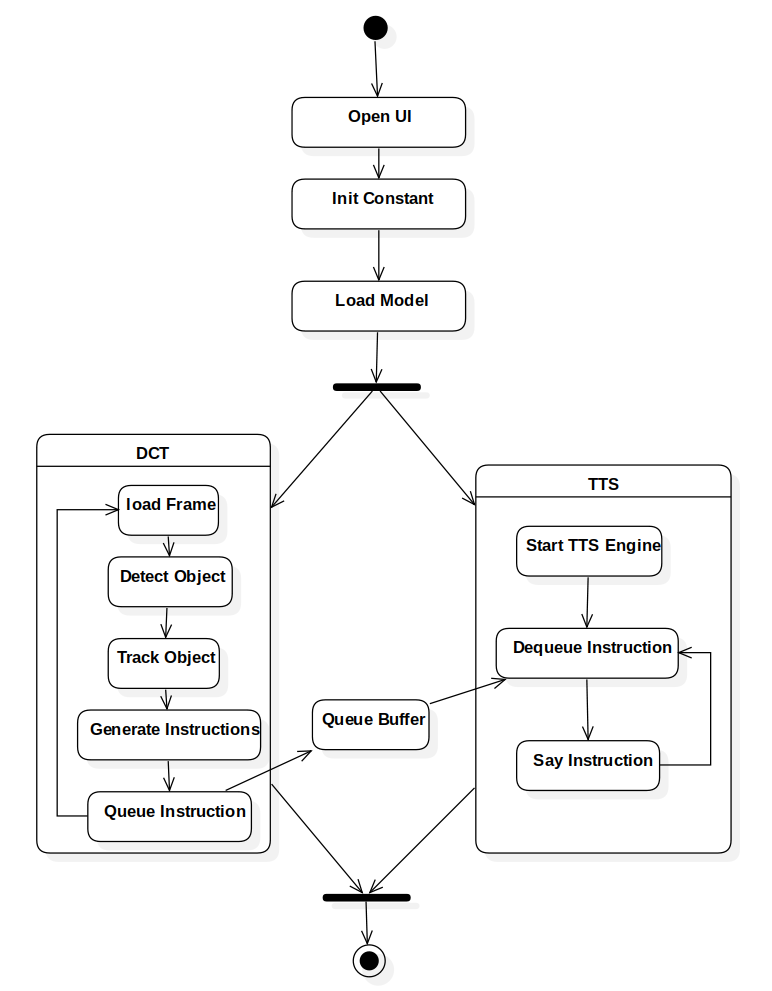
\includegraphics[scale=0.55]{img/System-Block-Diagram.png}
                \caption{System Block Diagram}
                \label{fig:System Block Diagram}
            \end{figure}
            \break
            The person will carry a systemin android phone . When the application is opened, it will access the camera. The camera will capture the video in real time with certain frame per second. Objects in each selected frame will be detected and recognized with the help of YOLO(You Only Look Once ) algorithm. It will give what object and where the obect is located in the image. The object is tracked using deepsort algorithm for tracking same object over following frames. Then, according to the object detected and their movement, a voice guidance is provided so that the person is made known about the object and be able to dodge the object instead of colliding with it.
        \section{YOLO - You Only Look Once}
            \subsection{What is YOLO?}
                YOLO stands for You Only Look Once. It's a object detector that uses features learned by a Deep Convolutional Network(DFN) to detect an object. YOLO makes use of only Convolutional Layers.   
            \subsection{Feature of YOLO}
                Some of the features of YOLO is given below:
                \begin{itemize}
                    \item It has 75 convolutional layer.
 	                \item It does not have any form of pooling.
 	                \item YOLO is invariant to size of input image yet, we stick on constant input size.
 	                \item The network downsample image by a factor called stride of network.

                        \tab for eg. If the stride of network is 32.

                        \tab input size = 416*416

                        \tab then, Output size = 13*13
                         
                        \tab Output size is stride times smaller than input size.
                         
                \end{itemize}
                
            \subsection{Interpreting the Result}
                The output of the YOLO object detection is a feature map. Each cell in the output image can predict a fixed number of bounding boxes. The YOLOV3 produces 3 bounding box for each cell.
                In feature map, we've B *(5+C) entries in feature map.\\
                \tab where,

                    \tab \tab B represents the number of bounding box each cell can predict. 

                    \tab \tab Each bounding box have 5+C attributes,

                        \tab \tab \tab here, C represents class confidence for each bounding box.
                        
                        \tab \tab Extra 5 is for\\
                            \tab \tab \tab $t_x$ for box co-ordinate\\
                            \tab \tab \tab $t_y$ for box co-ordinate\\
                            \tab \tab \tab $t_w$ for box co-ordinate\\
                            \tab \tab \tab $t_h$ for box co-ordinate\\
                            \tab \tab \tab $p_o$ for Objectness score\\
                Each cell of a feature map predict an object through one of it's bounding box. One Bounding box is responsible for detecting only one given objects.
                
            \subsection{How we do?}
                Consider, \\
                    \tab Image Size = 416*416\\
		            \tab stride = 32\\
		            \tab Output Image = 13 * 13 is Image of 13*13 cells\\
		        Each cell gives feature map of  B * (5+C) entries.\\
		    \begin{figure}[ht]
                \centering
                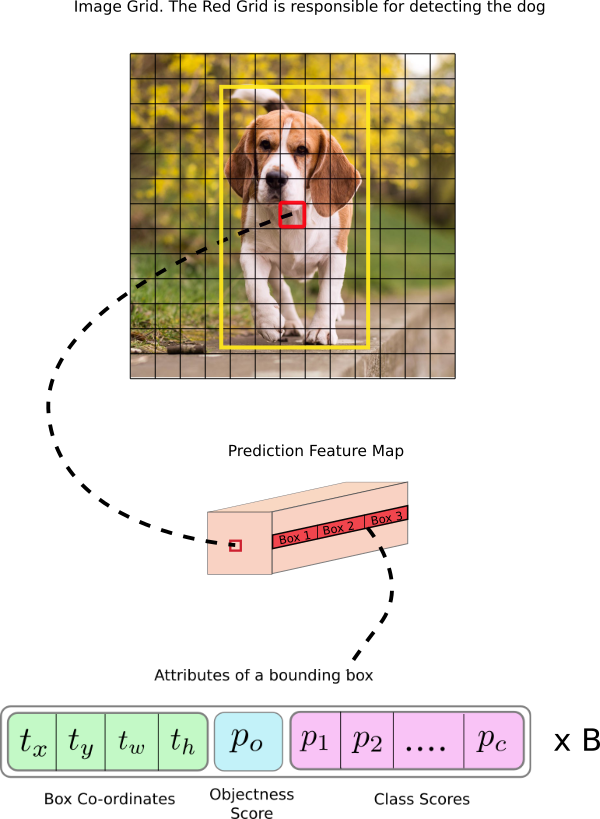
\includegraphics[scale=0.4]{img/yolo-5.png}
                \caption{Feature map of each cell}
                \label{fig:}
            \end{figure}
		        \subsubsection{Objectness Score}
                    One of the 5 attribute $P_o$ is probability that the object is contained inside a bounding box.
                    
                        \tab $P_o$ is nearly equal to 1 if the object is contained. It mainly occurs at the center of ground truth box.
                        
                        \tab $P_o$ is nearly equal to 0 if the cell contain no object. It mainly occurs at the corners of ground truth box.
                            
                \subsubsection{Class Confidence}
                    Class Confidence in the bounding box are the probabilities of detected object belong to particular class. Before YOLOV3, soft max was used for the class score. In V3, Soft max was dropped and Sigmoid was adopted instead. It is because Soft max assumes classes are mutually exclusive. i.e. If an object belongs to one class, then it cannot belongs to another class(True only for COCO data set).It is not true when we've classes like women and person which are mutually inclusive.
            \subsection{Benefits of YOLO}
                \begin{itemize}
                    \item Fast and Good for real time processing
	                \item Predictions are made from one single network.
                \end{itemize}
                
            \subsection{YOLO Outputs}
                \begin{figure}[ht]
                    \centering
                    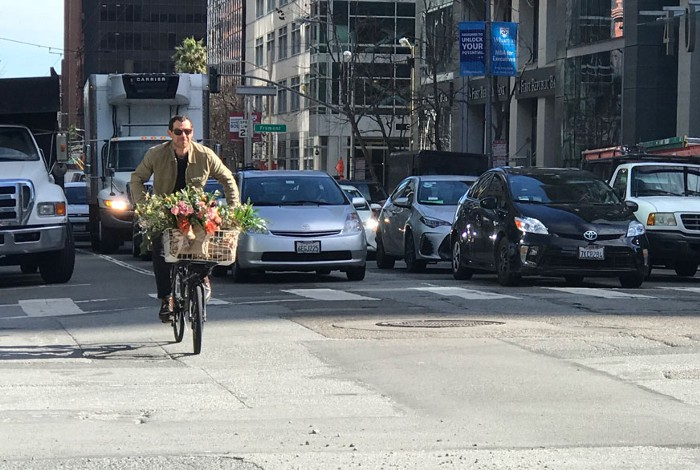
\includegraphics[scale=0.5]{img/testImage.jpeg}
                    \caption{Test image feeded to YOLO network}
                \end{figure}
                \break
                \begin{figure}[ht]
                    \centering
                    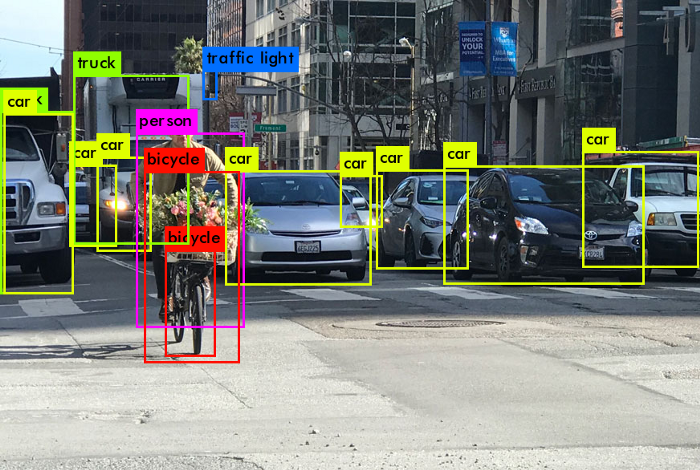
\includegraphics[scale=0.5]{img/PredictImage.png}
                    \caption{Output image from YOLO network}
                \end{figure}

            \subsection{YOLO v1 -- CNN Design}
                \begin{figure}[ht]
                    \centering
                    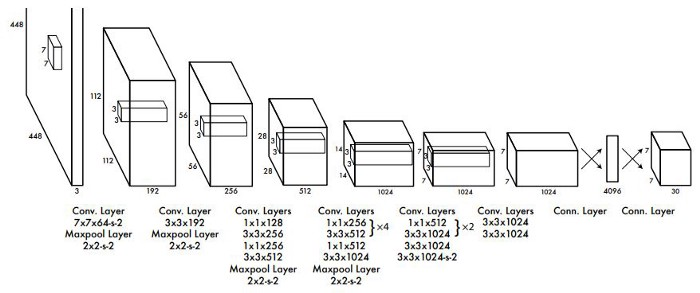
\includegraphics[width=1.0\textwidth]{img/yolov1_CNN-design.jpeg}
                    \caption{YOLO v1 CNN}
                    \label{fig:yolov1cnn}
                \end{figure}
                YOLO v1 CNN is shown in fig \ref{fig:yolov1cnn}.\cite{redmon2016you} It has 24 convolution layer followed by 2 fully connected layers that are responsible for classification of objects and regression of bounding boxes. Here, convolution layers acts as a feature extractor. The final output is 7 x 7 x 30 tensor. Leaky RelU activation function is used for all layers except the final layer. The final layer uses a linear activation function.
                \pagebreak
            \subsection{Loss Design}
                YOLO design uses sum squared error as the backbone of loss.\cite{redmon2016you} Since, multiple grid in the output do not contain any objects and their confidence score is zero. They overpower the gradients from a few cells that contain the objects. To avoid such overpower that leads to training divergence and model instability, YOLO increases the weight $(\lambda_{coord} = 5)$ for prediction from bounding box containing object and reduces the weight $\lambda_{noobj}=0.5$ for predictions from bounding boxes that do not contain any objects.

                \begin{equation}
                    \label{eqn:yolov1losspart1}
                    \lambda_{coord} \sum_{i=0}^{s^2} \sum_{j=0}^{B} \mathbbm{1}_{i j}^{obj} [(x_i-\hat{x_i})^2 + (y_i - \hat{y_i})^2]
                \end{equation}

                The equation \ref{eqn:yolov1losspart1} shows the first part of YOLO loss. It calculates the error in the prediction of center coordinates of bounding box. The loss function penalizes error in center coordinate of the bounding box, if the predictor is responsible for the ground truth box.

                \begin{equation}
                    \label{eqn:yolov1losspart2}
                    \lambda_{coord} \sum_{i=0}^{s^2} \sum_{j=0}^{B} \mathbbm{1}_{i j}^{obj} [(\sqrt{w_i}-\sqrt{\hat{w_i}})^2 + (\sqrt{h_i} - \sqrt{\hat{h_i}})^2]
                \end{equation}

                The equation \ref{eqn:yolov1losspart2} shows the second part of YOLO loss. It calculates the error in prediction of bounding box width and height. Here, if the magnitude of error in small bounding box is same as that of large bounding box. It is more wrong for small bounding box that a large bounding box. Hence, a square root of those values is used to calculate the loss. The loss function penalizes error in width and height of the bounding box, if the predictor is responsible for the ground truth box.


                \begin{equation}
                    \label{eqn:yolov1losspart3}
                    \sum_{i=0}^{s^2} \sum_{j=0}^{B} \mathbbm{1}_{i j}^{obj} (C_i-\hat{C_i})^2
                \end{equation}

                The equation \ref{eqn:yolov1losspart3} shows the third part of YOLO loss. It calculates the error in prediction of object confidence score for bounding boxes that have an object. The loss function only penalize object confidence score, if that predictor is responsible for the ground truth box. 

                \begin{equation}
                    \label{eqn:yolov1losspart4}
                    \lambda_{noobj}  \sum_{i=0}^{s^2} \sum_{j=0}^{B} \mathbbm{1}_{i j}^{obj} (C_i-\hat{C_i})^2
                \end{equation}

                The equation \ref{eqn:yolov1losspart4} shows the fourth part of the YOLO loss which calculates the error in prediction of object confidence score for bounding boxes that do not have an object.

                \begin{equation}
                    \label{eqn:yolov1losspart5}
                    \sum_{i=0}^{s^2} \mathbbm{1}_{i}^{obj} \sum_{c \in classes } (p_i(c)-\hat{p_i}(c))^2
                \end{equation}

                This equation \ref{eqn:yolov1losspart5} shows fifth part of YOLO loss. It calculates the error in prediction of class probabilities for grid cells that have an object. The loss funciton only penalizes class probabilities error, if an object is present in that grid cell.

                The loss function is:
                \begin{equation}
                    \begin{split}
                        \lambda_{coord} \sum_{i=0}^{s^2} \sum_{j=0}^{B} \mathbbm{1}_{i j}^{obj} [(x_i-\hat{x_i})^2 + (y_i - \hat{y_i})^2] \\
                        + \lambda_{coord} \sum_{i=0}^{s^2} \sum_{j=0}^{B} \mathbbm{1}_{i j}^{obj} [(\sqrt{w_i}-\sqrt{\hat{w_i}})^2 + (\sqrt{h_i} - \sqrt{\hat{h_i}})^2] \\ 
                        + \sum_{i=0}^{s^2} \sum_{j=0}^{B} \mathbbm{1}_{i j}^{obj} (C_i-\hat{C_i})^2 \\ 
                        + \lambda_{noobj}  \sum_{i=0}^{s^2} \sum_{j=0}^{B} \mathbbm{1}_{i j}^{obj} (C_i-\hat{C_i})^2 \\ 
                        + \sum_{i=0}^{s^2} \mathbbm{1}_{i}^{obj} \sum_{c \in classes } (p_i(c)-\hat{p_i}(c))^2
                    \end{split}
                \end{equation}
                $ \mathbbm{1}_{i,j}^{obj} $  is 1 when $j^{th}$ bounding box of $i^{th} $ grid has object, otherwise 0.
                \pagebreak
        \section{Intersection Over Union}
             \begin{figure}[ht]
                \centering
                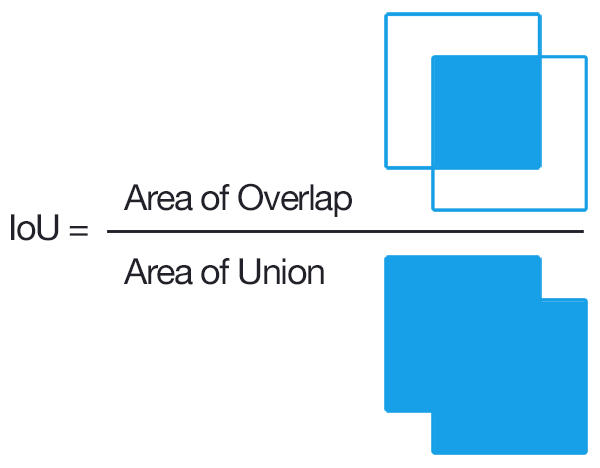
\includegraphics[width=0.90\textwidth]{img/IOU_1.png}
                \caption{Intersection Over Union }
            \end{figure}
            Intersection over union(IOU) is a measure of overlap between two bounding box. In computer vision it is used for correctly detecting an object. To know object detection first you have to know about object localization. Object localization refers to figuring out where is the object in the picture and showing it with rectangular box. IOU is known to be a good metric for measuring overlap between two bounding boxes or masks. \\
            Following pictures shows what is goodness measure of IOU \\
            \begin{figure}[ht]
                \centering
                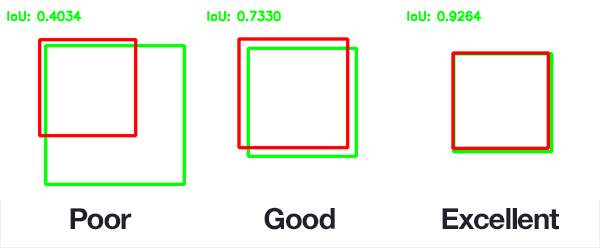
\includegraphics[width=0.90\textwidth]{img/IOU_3.png}
                \caption{Goodness measure of IOU}
            \end{figure}
            Informally, IOU measures how equal two areas are. In terms of size and location of the area. If two areas are exactly equal, IOU will be 1. If two areas are far apart, even if their shape is same, they will have IOU 0. And if two areas lie at the same location but their size differs a lot, then also IOU will be a small value.\cite{sheremet_2020}
            \begin{figure}[ht]
                \centering
                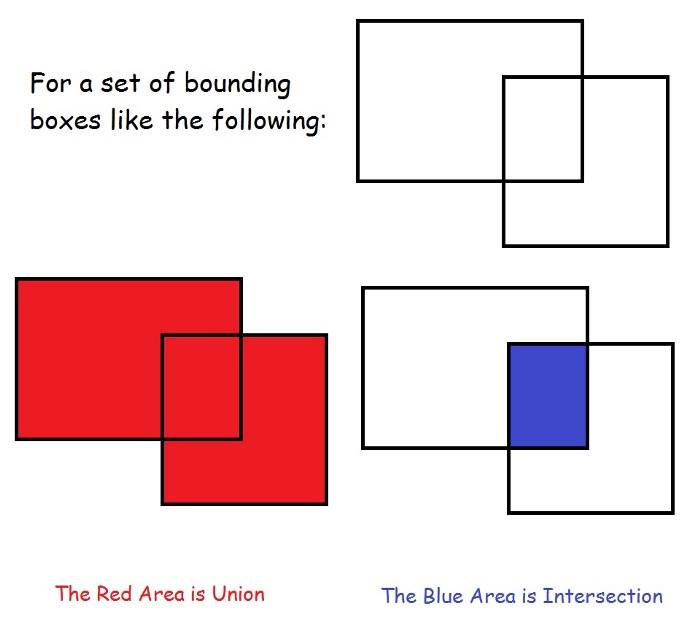
\includegraphics[width=0.90\textwidth]{img/IOU_2.jpg}
                \caption{Bounding Box Union and Intersection}
            \end{figure}
            $$ IOU(Box1, Box2) = \frac{Intersection_Size(Box1, Box2)}{Union_Size(Box1, Box2)}  $$
            \pagebreak
        \section{Non-Maximum Suppression}
            \begin{figure}[ht]
                \centering
                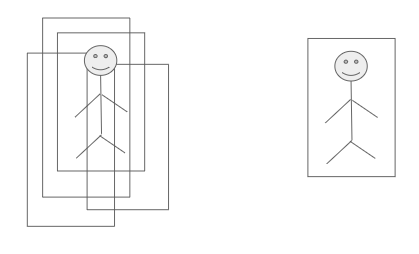
\includegraphics[width=0.85\textwidth]{img/NMS_2.png}
                \caption{Non Maximum Suppression}
            \end{figure}
            Non Maximum Suppression (NMS) is a technique used in many computer vision algorithms. It is a class of algorithms to select one entity (e.g. bounding boxes) out of many overlapping entities. The selection criteria can be chosen to arrive at particular results. Most commonly, the criteria is some form of probability number along with some form of overlap measure (e.g. IOU). 

            In object detection, there is a problem that an algorithm detects multiple bounding boxes for a single object. To solve this problem there, is a technique called non-max supression.Non-max suppression cleans up the multiple detection and end with just one detection per object. For this it chooses the bounding box with highest probability and suppressed all the other bounding boxes who’s IOU with it is greater, so in last only one bounding box is left which is more accurate.\cite{k_2019}\\
            \textbf{Input}: A list of Proposal boxes B, corresponding confidence scores S and overlap threshold N. \\
            \textbf{Output}: A list of filtered proposals D. \\
            \textbf{Algorithm: }
            \begin{enumerate}
                \item Select the proposal with highest confidence score, remove it from B and add it to the final proposal list D. (Initially D is empty). 
                \item Now compare this proposal with all the proposals — calculate the IOU (Intersection over Union) of this proposal with every other proposal. If the IOU is greater than the threshold N, remove that proposal from B.
                \item Again take the proposal with the highest confidence from the remaining proposals in B and remove it from B and add it to D. 
                \item Once again calculate the IOU of this proposal with all the proposals in B and eliminate the boxes which have high IOU than threshold. 
                \item This process is repeated until there are no more proposals left in B 
            \end{enumerate}
            \begin{figure}[ht]
                \centering
                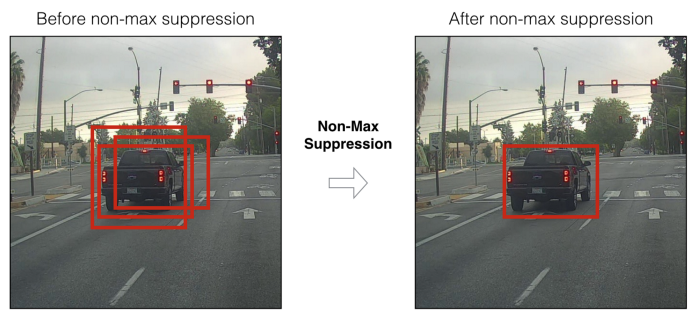
\includegraphics[width=0.90\textwidth]{img/NMS_1.png}
                \caption{Result before and after Non-max Suppression}
            \end{figure}
            Most object detection algorithms use NMS to whittle down a large number of detected rectangles to a few. The need for NMS arises because of the way object detection works in most cases ( e.g. Faster RCNN, Yolo V3, SSD, etc). At the most basic level, most object detectors do some form of windowing. Many, thousands, windows of various size and shapes are generated either directly on the image or on a feature of the image ( e.g. after a deep CNN such as ResNet). These windows supposedly contain only one object, and a classifier is used to obtain a probability/score for each classes. Once the detector outputs the large number of bounding boxes, it is necessary to pick the best ones. NMS is the most commonly used algorithm for this task. In essence it is a form of clustering algorithm. Attempts have been made to use standard clustering algorithms such as k-means, Nearest Neighbor, DB Scan, etc. in object detection.
            \pagebreak
        \section{Kalman Filter in Deepsort}
            The most popular and one of the most widely used, elegant object tracking framework is Deep SORT, an extension to SORT (Simple Real time Tracker). 
                
            
            The Kalman filter keeps track of the system and the variance or uncertanity of the estimate. The estimate is updated using a state transition model and measurements.
            \begin{figure}[ht]
                \centering
                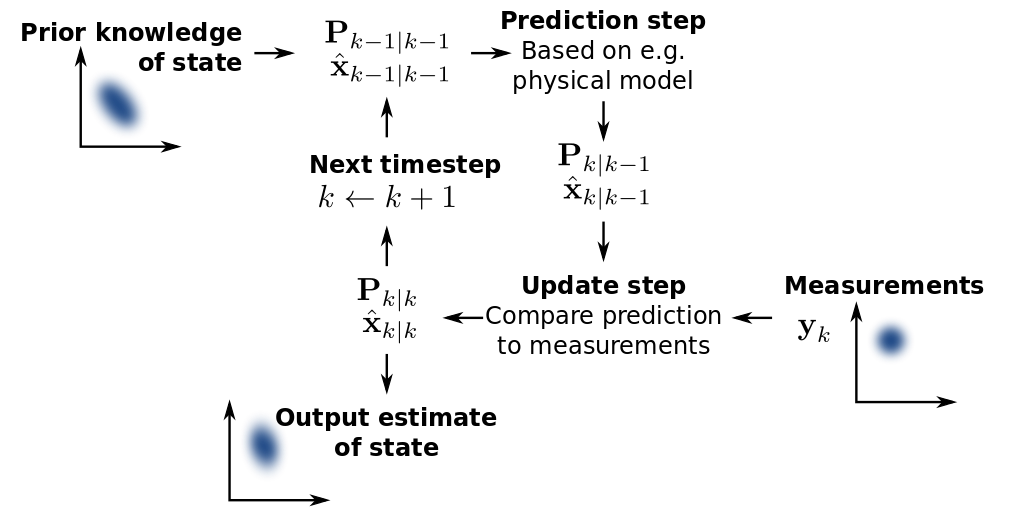
\includegraphics[scale=0.4]{img/kalman.png}
                \caption{Kalman Filter}
                \label{fig:Feature of COCO dataset}
            \end{figure}


            ${\hat {x}}_{k\mid k-1}$ denotes the estimate of the system's state at
            time step k before the k-th measurement ${y_k}$ has been taken into
            account;$P_{k\mid k-1}$ is the corresponding uncertainty.
                        
            \begin{figure}[ht]
                \centering
                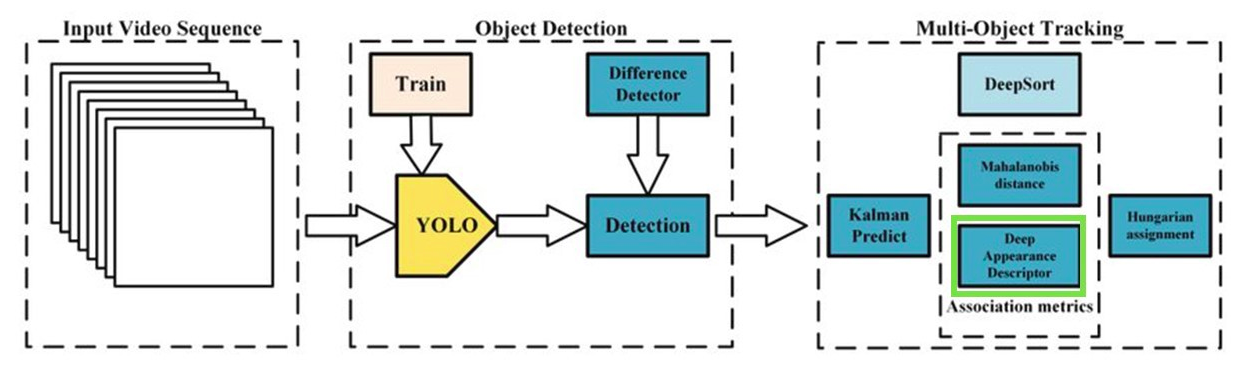
\includegraphics[scale=0.4]{img/deep_sort.png}
                \caption{YOLO with Kalman Filter}
                \label{fig: Deepsort algorithm}
            \end{figure}
            \pagebreak

        \section{Threads Implementation in Desktop}
            There were basically two modules in the inference system which were DCT module and TTS module. To bring synchronization between those two modules, threads was implemented which let those two modules run side by side.\\
            The main logic was the use of a buffer variable: command list in which the DCT module stores the information to be given to the user and the TTS module actually executes the information.\\
            In actual programme, the main module is DCT module which calls TTS modules in a threads. In DCT module:
\begin{verbatim}
self.thread = TTS()
self.thread.start()
self.thread.setLanguage(False)
\end{verbatim}
            To test the threads, a test program was made to make sure it works in which simply two audio files were played side by side:
\begin{verbatim}
import threading
import time
import playsound
song = "1.mp3"
class myThread (threading.Thread):
    def __init__(self, song_name):
        threading.Thread.__init__(self)
        self.song_name = song_name
    def run(self):
        playsound.playsound(self.song_name)
thread1 = myThread("1.mp3")
thread2 = myThread("2.mp3")
thread1.start()
thread2.start()
print("Exiting Main Thread")
\end{verbatim}
            As output, we get two audio files playing side by side at a same time.

        \section{Region Detector}
        Region detector gets ROI and Frame from the inference system and returns the region(left, center or right) on which the ROI lies.
        The steps involved are:
            \begin{itemize} 
                \item Region detector gets: Frame width , Frame height and  ROI(Region Of Interest) coordinates from the inference system.
                \item Then the detector calculates the coordinates for left, center and right region.
\begin{verbatim}
right = [0,0,int(self.width/3),self.height]
center = [int(self.width/3),0,int(self.width/3*2),self.height]
left = [int(self.width/3*2),0,int(self.width),self.height]
\end{verbatim}
                \item Then it finds intersection of ROI with each of the left, right and center region and select the miximum one.
\begin{verbatim}
l = [ ]
l.append(self.intersection(center,self.roi))
l.append(self.intersection(left,self.roi))
l.append(self.intersection(right,self.roi))
return l.index(max(l))
\end{verbatim}
                \item The maximum intersection gives the region on which the ROI lies.
            \end{itemize}
        \section{Command Index Generation(CIG) for TTS}
            Command index generation generates the index of the command to be executed for the detected object.\\The object classes as recognized by the class index are:
\begin{verbatim}
    ['car','truck','bus','person','bicycle','motorbike']      
\end{verbatim}
            And the commands as recognized by command index are:
\begin{verbatim}
    ['car ahead',
    'car in your left',
    'car in your right',
    'Truck ahead',
    'Truck in your left',
    'Truck in your right',
    'Bus ahead',
    'Bus in your left',
    'Bus in your right', 
    'person ahead', 
    'person in your left', 
    'person in your right',
    'Bicycle ahead', 
    'Bicycle in your left',
    'Bicycle in your right', 
    'Bike ahead', 
    'Bike in your left',
    'Bike in your right']
\end{verbatim}
            After getting region value from Region Detector and class index value from inference system, CIG now calculates the actual index of the command using the formula:
\begin{verbatim}
    command_index = class_index * 3 + regionValue()
\end{verbatim}
            Now, with command index value, TTS module can execute the required command.
        \section{Text to Speech (pyttsx3)}
	        Text to speech conversion is simply done by using pyttsx3 library which uses pre-installed text to speech synthesizer engine to formulate text given as input then generating audio file as output.
	        here, Included TTS engines:
            \begin{itemize}
                \item sapi5
                \item espeak
                \item libspeak
                \item festival
            \end{itemize}
            The text-to-speech (TTS) synthesis procedure consists of two main phases.
            \\Namely: 
                \begin{description}
                    \item[Generation of linguistic representation:] The input text is transcribed into a phonetic or some other linguistic representation
                    \item[Generation of speech waveforms:] The output is produced from this phonetic and prosodic information
                \end{description}
            The character string is then pre-processed and analysed into phonetic representation which is usually a string of phonemes with some additional information for correct intonation, duration, and stress.  Finally the audio file is generated as the calculated parameters of speech from the TTS engines for the audible result to user.
            \pagebreak
        \section{Detection Evaluation}
            Evaluation for output of Detection is done using F1 Score analysis. It is determined from confusion matrix as:\\\\
            \begin{figure}[h]
                \centering
                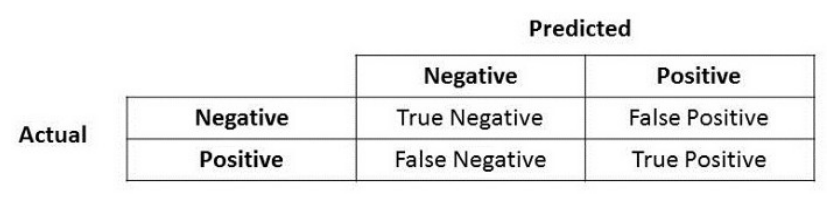
\includegraphics[width=0.90\textwidth]{img/confusion_matrix.png}
                \caption{Confusion Matrix}
            \end{figure}\\\\
            \textbf{True Positive (TP):}\\
                Number of Correct Detections in each frame.\\\\
            \textbf{False Positive (FP):}\\
                Number of Wrong Detection in each frame.\\\\
            \textbf{False Negative (FN):}\\
                Number of Missed Detection in each frame.\\\\
            \textbf{Precision:}\\
                Precision is a good measure to determine, when the costs of False Positive is high. Precision talks about how precise/accurate a model is out of those predicted positive, how many of them are actual positive. The denominator is the Total Predicted Positive.
                $$Precision =\frac{TP}{TP+FP}=\frac{TP}{Total Predicated Positive}$$\\
            \textbf{Recall:}\\
                Recall actually calculates how many of the Actual Positives our model capture through labeling it as Positive (True Positive). 
                $$Recall =\frac{TP}{TP+FN}=\frac{TP}{Total Actual Positive}$$\\
            \textbf{F1 Score:}\\
                F1 is a function of Precision and Recall. F1 Score is needed when you want to seek a balance between Precision and Recall.\\
                $$F1 Score = \frac{2 * Precision * Recall}{Precision + Recall}$$
                \pagebreak
        \section{MOT Evaluation}            
            \subsection{Metrics}            
                Typical evaluation format is shown as:\\             
                IDF1| IDP| IDR| Rcll| Prcn| FAR| GT| MT| PT| ML| FP| FN| IDs| FM| MOTA| MOTP| MOTAL\\\\
                The meaning of each alias is\\
                \textbf{IDF1(ID F1 Score):}\\
                $$IDF1=\frac{2 *IDTP} {2 * IDTP + IDFP + IDFN}$$
                \textbf{IDP(ID Precison):}\\
                $$IDP=\frac{IDTP}{IDTP +IDFP}$$                
                \\\textbf{IDR(ID Recall):}\\
                $$IDR = \frac{IDTP}{IDTP +IDFN}$$
                \\\textbf{IDTP:}\\
                The longest associated trajectory matching to a groundtruth trajectory is regarded as the gt's true ID.\\
                Then other trajectories matching to this gt is regarded as a 'IDFP'.\\
                \\\\\\\textbf{Rcll(Recall):}\\
                The ratio of TP boxes to GT boxes.\\
                $$Recall=\frac{TP}{TP + FN}$$\\
                \\\textbf{Prcn(Precision):}\\
                The ratio of TP boxes to all detected boxes.\\
                $$Precision=\frac{TP}{TP + FP}$$\\
                \\\textbf{FAR(False Alarm Ratio):}\\
                The ratio of FP boxes to frame number.\\
                $$FAR=\frac{FP}{\sum_t 1}$$\\
                \\\textbf{GT(Number of GroundtruthTrajectory):}\\
                The number of groundtruth trajectories.\\
                \\\textbf{MT(Number of Mostly Tracked Trajectory):}\\
                The number of trajectories that have over 80\% target tracked.\\
                \\\textbf{PT(Number of Partially Tracked Trajectory):}\\
                The number of trajectories that have 20\% to 80\% target tracked.\\
                $$PT= GT - MT - ML$$\\ 
                \\\textbf{ML(Number of Mostly Lost Trajectory):}\\
                The number of trajectories that have less than 20\% target tracked. Total false positive number among all frames.\\
                $$FP=\sum_t \sum_i {fp}_{i, t}$$\\
                \\\textbf{FN(Number of False Negatives):}\\ 
                Total false negative number among all frames.\\
                $$FN=\sum_t \sum_i fn_{i, t}$$\\
                \\\\\\\textbf{IDs(Number of IDSwitch):}\\
                ID switch number, indicating the times of ID jumps.\\
                $$IDs=\sum_t ids_{i, t}$$\\
                \\\textbf{FM(Number of Fragmentations):}\\
                ID switch is the special case of fragmentation when ID jumps. Fragmentation reflects the continousity of trajectories. When trajectories are determinated, it counts all missed target in
                each frame.\\
                \\\textbf{MOTA(Number of Multiple Object Tracking Accuracy):}\\
                A metric reflects the tracking accuracy. It has intergrated consideration of FN, FP, and IDS.\\
                $$T=\sum_t \sum_i gt_{i,t}$$\\
                $$MOTA=1 - \frac{FN + FP + IDS}{T}$$\\
                \\\textbf{MOTP(Number of Multiple Object Tracking Precision):}\\
                A metric reflects the tracking precision. \\
                $$MOTP=\frac{\sum_{i,t}IoU_{t, i}}{TP}$$\\
                \\\textbf{MOTAL(MOTA Log):}\\
                $$MOTAL= 1 - \frac{FN + FP + \log_{10}IDS}{T}$$ 

        